%===================================================================================
% Chapter: Proposed Solution
%===================================================================================
\chapter{Propuesta de Solución}\label{chapter:proposed-solution}
Esta investigación busca poder expresar un corpus anotado a través de una ontología definida, generando un grafo de conocimiento como resultado. Otro de los objetivos claros, es poder hacer esto mediante un algoritmo computacional, el cual debe ser, además, finito y determinista. 

%===================================================================================

% \section{Primeros pasos}
% Primeramente debemos hacer algunas definiciones sobre las cuales nos basaremos en lo adelante. Estas son {\it algoritmo}, {\it algoritmo computacional}, {\it algoritmo finito} y {\it algoritmo determinista}.

% \begin{definition}
% 	Un \textbf{algoritmo} es un conjunto finito y ordenado de instrucciones bien definidas y estructuradas que nos permite llevar a cabo una tarea o encontrar la solución a un determinado problemas.
% \end{definition}

% \begin{definition}
% 	Un \textbf{algoritmo computacional} es un algoritmo que puede ser programado en una máquina de cómputo.
% \end{definition}

% \begin{definition}
% 	Un \textbf{algoritmo finito} es un algoritmo que termina luego de ejecutar una cantidad finita de instrucciones.
% \end{definition}

% \begin{definition}
% 	Un \textbf{algoritmo determinista} es un algoritmo finito que produce el mismo resultado siempre que tenga la misma entrada. Además, la \guillemot{\texttt{máquina interna}} pasará siempre por la misma secuencia de estados, o un poco más informal, la secuencia de instrucciones y resultados de las mismas será siempre igual.
% \end{definition}

\section{Analizador sintáctico}
Primeramente, es necesaria la creación de una herramienta capaz de fragmentar en objetos con significado computacional el contenido de los archivos de anotación escritos con el formato visto en la sección \ref{section:annotation_file_format}. Esta herramienta asume que el archivo está correctamente escrito, tomando en cuenta las reglas explicadas en las propia sección \ref{section:annotation_file_format}. El algoritmo \ref{algorithm:annotation_file_parsing} escrito en pseudocódigo muestra cómo se puede llevar a cabo esta tarea.

El algoritmo \ref{algorithm:annotation_file_parsing} se apoya en la implementación de algunas funciones previas. Ellas son \textit{ParseTextAnnotation}, \textit{ParseTextAnnotation}, \textit{ParseRelationAnnotation}, \textit{ParseSameAsRelationAnnotation}, \textit{ParseAttributeAnnotation} y por último, en caso de que se quieran procesar los comentarios, se usa \textit{ParseCommentAnnotation}. Estas funciones son usadas para analizar sintácticamente las anotaciones de texto, relación, relación de igualdad definida con el identificador `*', atributos y comentarios respectivamente. Estas funciones pueden llevarse a cabo mediante el uso de expresiones regulares para obtener los fragmentos de cada tipo en cada una de las anotaciones. A continuación se presentan las posibles expresiones regulares a usar aclarando que estas no son las únicas que existen para resolver este problema.

\begin{annexample}
[backgroundcolor=white]
{5.54in}
{fig:text_annotation_regular_expression}
{Expresión regular para la comprensión de la anotación de texto}
{Expresión regular para la comprensión de la anotación de texto.}
	\ttfamily
	\StartingRegex\GroupRegex{T\BracketRegex{0-9}\OneOrMoreRegex}$\backslash$t\,\GroupRegex{\BracketRegex{A-Za-z}\OneOrMoreRegex} \GroupRegex{\BracketRegex{0-9}\OneOrMoreRegex\space\BracketRegex{0-9}\OneOrMoreRegex\GroupRegex{;\BracketRegex{0-9}\OneOrMoreRegex\space\BracketRegex{0-9}\OneOrMoreRegex}\ZeroOrMoreRegex} \GroupRegex{.\OneOrMoreRegex}\EndingRegex
\end{annexample}

De la expresión regular de la figura \ref{fig:text_annotation_regular_expression} podemos extraer la siguiente información de las anotaciones de relación:
\begin{itemize}
	\item[•] \texttt{T\BracketRegex{0-9}\OneOrMoreRegex} $\longrightarrow$ identificador de esta anotación
	\item[•] \texttt{\BracketRegex{A-Za-z}\OneOrMoreRegex} $\longrightarrow$ tipo de rol
	\item[•] \texttt{\BracketRegex{0-9}\OneOrMoreRegex\space\BracketRegex{0-9}\OneOrMoreRegex\GroupRegex{;\BracketRegex{0-9}\OneOrMoreRegex\space\BracketRegex{0-9}\OneOrMoreRegex}\ZeroOrMoreRegex} $\longrightarrow$ rango de posiciones
	\item[•] \texttt{.\OneOrMoreRegex} $\longrightarrow$ texto anotado
\end{itemize}

\begin{annexample}
[backgroundcolor=white]
{5.04in}
{fig:relation_annotation_regular_expression}
{Expresión regular para la comprensión de la anotación de relación}
{Expresión regular para la comprensión de la anotación de relación.}
	\ttfamily
	\StartingRegex\GroupRegex{R\BracketRegex{0-9}\OneOrMoreRegex}$\backslash$t\,\GroupRegex{\BracketRegex{A-Za-z$\backslash$-}\OneOrMoreRegex} Arg1:\GroupRegex{T\BracketRegex{0-9}\OneOrMoreRegex}\space Arg2:\GroupRegex{T\BracketRegex{0-9}\OneOrMoreRegex}\EndingRegex
\end{annexample}

De la expresión regular de la figura \ref{fig:relation_annotation_regular_expression} podemos extraer la siguiente información de las anotaciones de relación:
\begin{itemize}
	\item[•] \texttt{R\BracketRegex{0-9}\OneOrMoreRegex} $\longrightarrow$ identificador de esta anotación
	\item[•] {\tt\BracketRegex{A-Za-z$\backslash$-}\OneOrMoreRegex} $\longrightarrow$ tipo de relación
	\item[•] \texttt{T\BracketRegex{0-9}\OneOrMoreRegex} $\longrightarrow$ son los argumentos de la relación
\end{itemize}

\begin{annexample}
[backgroundcolor=white]
{3.27in}
{fig:same_as_relation_annotation_regular_expression}
{Expresión regular para la comprensión de la anotación de relación \textit{same-as}}
{Expresión regular para la comprensión de la anotación de relación \textit{same-as}.}
	\ttfamily
	\StartingRegex*$\backslash$t\,same-as \GroupRegex{T\BracketRegex{0-9}\OneOrMoreRegex}\GroupRegex{ \GroupRegex{T\BracketRegex{0-9}\OneOrMoreRegex}}\OneOrMoreRegex\EndingRegex
\end{annexample}

De la expresión regular de la figura \ref{fig:same_as_relation_annotation_regular_expression} podemos extraer la siguiente información de las anotaciones de relación \textit{same-as}:
\begin{itemize}
	\item[•] \texttt{T\BracketRegex{0-9}\OneOrMoreRegex} $\longrightarrow$ argumentos de esta anotación
\end{itemize}

\begin{annexample}
[backgroundcolor=white]
{3.16in}
{fig:attribute_annotation_regular_expression}
{Expresión regular para la comprensión de la anotación de atributo}
{Expresión regular para la comprensión de la anotación de atributo.}
	\StartingRegex\GroupRegex{A\BracketRegex{0-9}\OneOrMoreRegex}$\backslash$t\GroupRegex{\BracketRegex{A-Za-z}\OneOrMoreRegex} \GroupRegex{T\BracketRegex{0-9}\OneOrMoreRegex}\EndingRegex
\end{annexample}

De la expresión regular de la figura \ref{fig:attribute_annotation_regular_expression} podemos extraer la siguiente información de las anotaciones de relación \textit{same-as}:
\begin{itemize}
	\item[•] \texttt{A\BracketRegex{0-9}\OneOrMoreRegex} $\longrightarrow$ identificador de esta anotación
	\item[•] \texttt{\BracketRegex{A-Za-z}\OneOrMoreRegex} $\longrightarrow$ tipo de atributo
	\item[•] \texttt{T\BracketRegex{0-9}\OneOrMoreRegex} $\longrightarrow$ identificador de la anotación de texto que se modifica
\end{itemize}

\begin{annexample}
[backgroundcolor=white]
{1.7in}
{fig:attribute_relation_annotation_regular_expression}
{Expresión regular para la comprensión de la anotación de atributo}
{Expresión regular para la comprensión de la anotación de atributo.}
	\StartingRegex\GroupRegex{\#\BracketRegex{0-9}\ZeroOrMoreRegex} \GroupRegex{.\ZeroOrMoreRegex}\EndingRegex
\end{annexample}

De la expresión regular de la figura \ref{fig:attribute_annotation_regular_expression} podemos extraer la siguiente información de las anotaciones de relación \textit{same-as}:
\begin{itemize}
	\item[•] \texttt{\#\BracketRegex{0-9}\ZeroOrMoreRegex} $\longrightarrow$ identificador de esta anotación
	\item[•] \texttt{.\ZeroOrMoreRegex} $\longrightarrow$ comentario
\end{itemize}

\begin{algorithm}[H]
	\caption[Analizador sintáctico]{Analizador sintáctico.}\label{algorithm:annotation_file_parsing}
	\Function{ParseDocument}{
		\Input{document}
		\Output{list of annotations}
		\BlankLine
		\DefineCommand \textit{annotations}: \textnormal{list of annotations}\\
		$\assignment{annotations}{\varnothing}$\\
		\ForEach{line \InCommand document}{
			\If{$line\neq\varnothing$}{
				$\assignment{annotation}{ParseLine($line$)}$\\
				$annotations$.Append($annotation$)
			}
		}
		\Return{annotations}
	}
	\BlankLine
	\Function{ParseLine}{
		\Input{line}
		\Output{annotation}
		\BlankLine
		\DefineCommand \textit{first\_char}: \textnormal{character}\\
		$\assignment{first\_char}{line.FirstChar()}$\\
		\Switch{$first\_char$}{
			\Case{`T'}{
				\Return{\textnormal{ParseTextAnnotation($line$)}}
			}
			\Case{`R'}{
				\Return{\textnormal{ParseRelationAnnotation($line$)}}
			}
			\Case{`*'}{
				\Return{\textnormal{ParseSameAsRelationAnnotation($line$)}}
			}
			\Case{`A'}{
				\Return{\textnormal{ParseAttributeAnnotation($line$)}}
			}
			\Case{`\#'}{
				\Return{\textnormal{ParseCommentAnnotation($line$)}}
			}
			\Other{
				\ErrorCommand\textit{``No se identifica el tipo de anotación.''}
			}
		}
	}
\end{algorithm}

\section{Grafo de conocimiento}
Una vez que se haya analizado sintácticamente todo el corpus, se tendrá la información de las anotaciones en objetos computacionales y será más sencillo el trabajo con estos. En aras de evitar ambigüedades y concentrar el conocimiento para un mejor entendimiento de este y a la misma vez, poder facilitar la tarea de extraerlo de este grafo por un equipo de cómputo, el texto anotado es normalizado. Este texto se normaliza teniendo en cuenta las palabras que lo componen, y anotando en su lugar la palabra primitiva de esta. Por ejemplo, la palabra \guillemot{\texttt{sangramiento}} será anotada como \guillemot{\texttt{sangrar}} y la frase \guillemot{\texttt{glóbulos rojos}} como \guillemot{\texttt{glóbulo rojo}}.

Como se vio en la sección \ref{section:annotation_structure}, es necesario aclarar que hay que darle un orden a la creación de los nodos y aristas en este grafo, pues las propias anotaciones de texto y las relaciones tienen un orden implícito entre ellas. Por ejemplo, en la propia figura \ref{fig:annotation_example_composing_concepts}, se debe procesar primero el rol ejercido por \guillemot{\texttt{problemas}} y por \guillemot{\texttt{cumpla}} antes de poder procesar \guillemot{\texttt{impiden}}; de lo contrario, el conocimiento descrito por \guillemot{\texttt{impiden}} quedaría incompleto o mal representado.

\subsection{Orden topológico}
El orden establecido por el modelo de anotación visto en el capítulo \ref{chapter:annotation_model} es un orden topológico. Para ello se tiene en cuenta el siguiente orden:

\begin{enumerate}
	\label{enum:knowledge_graph_build_order}
	\item Texto
	\item Atributos
	\item Relaciones de acción, predicado y contextualización
	\item Relaciones taxonómicas y de causa e implicación
\end{enumerate}

Es válido aclarar que una vez divididas las relaciones en estos tres grupos, estas son asociadas nuevamente, esta vez teniendo en cuenta la parte izquierda de cada una de ellas (\texttt{Arg1} en el archivo de anotación). Se crea un nodo por cada una de estas agrupaciones, un nodo creado en un nivel más avanzado teniendo en cuenta el orden visto anteriormente, representa una mayor cantidad de información y al mismo tiempo, información más específica respecto a su nodo asociado en niveles anteriores.

En la figura \ref{fig:text_document1} puede verse un ejemplo de documento de texto, en la \ref{fig:annotated_document1} se ve el documento anotado asociado a este, y en la \ref{fig:knowledge_graph1.3} se puede ver cómo queda el grafo de conocimiento resultante de este corpus. En este caso el corpus es un solo documento con una única oración, pero en la práctica un corpus tendrá muchos más documentos y más oraciones en cada uno de ellos. La flecha que puede haber en algunas líneas del ejemplo significa que esta línea en el documento es muy larga para ser mostrada en una única línea en el ejemplo y se continuará escribiendo debajo. En estos ejemplos, las palabras o frases no son normalizadas para un mejor entendimiento en lenguaje natural y además, porque hay varias formas, métodos y decisiones de cómo normalizar palabras o frases.
\begin{annexample}
[backgroundcolor=black!5]
{\textwidth}
{fig:text_document1}
{Ejemplo 1: documento \doublequote{\texttt{desmayo.txt}}}
{Ejemplo 1: documento \doublequote{\texttt{desmayo.txt}}.}
	El desmayo (o síncope) es una pérdida temporal de la {\scriptsize $\hookrightarrow$}\\
	conciencia.
\end{annexample}

\begin{annexample}
[backgroundcolor=cyan!13]
{\textwidth}
{fig:annotated_document1}
{Ejemplo 1: documento \doublequote{\texttt{desmayo.ann}}}
{Ejemplo 1: documento \doublequote{\texttt{desmayo.ann}}.}
	\# Sentence 1: El desmayo (o síncope) es una pérdida {\scriptsize $\hookrightarrow$}\\
	temporal de la conciencia.\\
	\# Keyphrases\\
	T1\space\space Concept 3 10\space\space\space\space desmayo\\
	T2\space\space Concept 14 21\space\space\space síncope\\
	T3\space\space Action 30 37\space\space\space\space pérdida\\
	T4\space\space Concept 38 46\space\space\space temporal\\
	T5\space\space Concept 53 63\space\space\space conciencia\\
	\# Relations\\
	R1\space\space is-a Arg1:T1 Arg2:T3\\
	R2\space\space in-context Arg1:T3 Arg2:T4\\
	R3\space\space target Arg1:T3 Arg2:T5\\
	\textasteriskcentered\space\space\space same-as T1 T2
\end{annexample}

Siguiendo el orden establecido \hyperref[enum:knowledge_graph_build_order]{anteriormente}, se puede ver en la figura \ref{fig:knowledge_graph1.1} el grafo de conocimiento resultante luego de realizado el punto $1$ es:

\begin{figure}[H]
	\begin{center}
		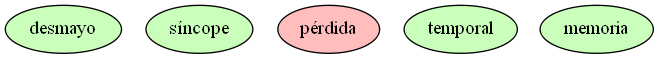
\includegraphics[width=4.4in]{graphics/knowledge_graph_example1_1.png}
		\caption[Ejemplo 1: grafo de conocimiento luego de realizado el punto 1]{Ejemplo 1: grafo de conocimiento luego de realizado el punto 1.}
		\label{fig:knowledge_graph1.1}
	\end{center}
\end{figure}

En el punto $2$ no hay nada que hacer con este corpus, pues no hay atributos, por tanto, el grafo de conocimiento quedará idéntico.

Para el punto $3$ son usadas las relaciones \texttt{R2} y \texttt{R3}, resultando:
\begin{figure}[H]
	\begin{center}
		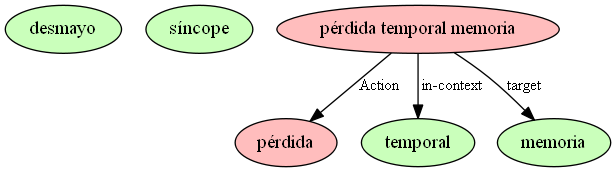
\includegraphics[width=5in]{graphics/knowledge_graph_example1_2.png}
		\caption[Ejemplo 1: grafo de conocimiento luego de realizado el punto 3]{Ejemplo 1: grafo de conocimiento luego de realizado el punto 3.}
		\label{fig:knowledge_graph1.2}
	\end{center}
\end{figure}

Para el punto $4$ son usadas las relaciones restantes, en este caso \texttt{R1} y \texttt{\textasteriskcentered}, resultando:
\begin{figure}[H]
	\begin{center}
		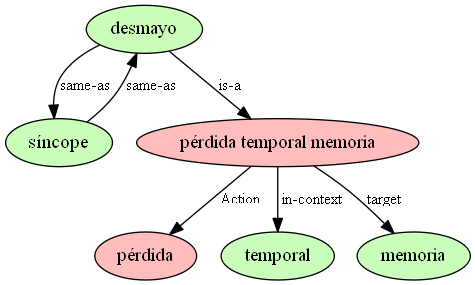
\includegraphics[width=3.8in]{graphics/knowledge_graph_example1_3.png}
		\caption[Ejemplo 1: grafo de conocimiento luego de realizado el punto 4]{Ejemplo 1: grafo de conocimiento luego de realizado el punto 4.}
		\label{fig:knowledge_graph1.3}
	\end{center}
\end{figure}

Por tanto, el grafo de conocimiento, dado el corpus de texto de la figura \ref{fig:text_document1} y la anotación de este como se muestra en la figura \ref{fig:annotated_document1}, está representado en la figura \ref{fig:knowledge_graph1.3}.

El ejemplo anterior es sencillo y muestra un documento con una única oración también sencilla. Ahora se muestra un ejemplo de un corpus que igualmente contiene un único documento con una única oración, pero esta vez, una oración más compleja y que abarca todos los grupos de relaciones que hay en el modelo de anotación.

\begin{annexample}
[backgroundcolor=black!5]
{\textwidth}
{fig:text_document2}
{Ejemplo 2: documento \doublequote{\texttt{higiene.txt}}}
{Ejemplo 2: documento \doublequote{\texttt{higiene.txt}}.}
	Las buenas prácticas de higiene, incluyendo lavarse las {\scriptsize $\hookrightarrow$}\\
	manos correctamente, pueden evitar infecciones.
\end{annexample}

\begin{annexample}
[backgroundcolor=cyan!13]
{\textwidth}
{fig:annotated_document2}
{Ejemplo 2: documento \doublequote{\texttt{higiene.ann}}}
{Ejemplo 2: documento \doublequote{\texttt{higiene.ann}}.}
	\# Sentence 1: Las buenas prácticas de higiene, incluyendo {\scriptsize $\hookrightarrow$}\\
	lavarse las manos correctamente, pueden evitar infecciones.\\
	\# Keyphrases\\
	T1\space\space Concept 4 10\space\space\space\space buenas\\
	T2\space\space Predicate 11 20 prácticas\\
	T3\space\space Concept 24 31\space\space\space higiene\\
	T4\space\space Action 44 51\space\space\space\space lavarse\\
	T5\space\space Concept 56 61\space\space\space manos\\
	T6\space\space Concept 62 75\space\space\space correctamente\\
	T7\space\space Action 84 90\space\space\space\space evitar\\
	T8\space\space Concept 91 102\space\space infecciones\\
	\# Relations\\
	R1\space\space in-context Arg1:T2 Arg2:T1\\
	R2\space\space domain Arg1:T2 Arg2:T3\\
	R3\space\space causes Arg1:T2 Arg2:T7\\
	R4\space\space is-a Arg1:T4 Arg2:T2\\
	R5\space\space target Arg1:T4 Arg2:T5\\
	R6\space\space in-context Arg1:T4 Arg2:T6\\
	R7\space\space target Arg1:T7 Arg2:T8\\
	\# Attributes\\
	A1\space\space Uncertain T7
\end{annexample}

Una vez más, siguiendo el orden establecido \hyperref[enum:knowledge_graph_build_order]{anteriormente}, se puede ver en la figura \ref{fig:knowledge_graph2.1} el grafo de conocimiento resultante luego de realizado el punto $1$ es:

\begin{figure}[H]
	\begin{center}
		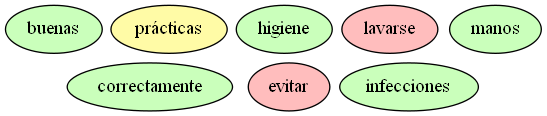
\includegraphics[width=4.2in]{graphics/knowledge_graph_example2_1.png}
		\caption[Ejemplo 2: grafo de conocimiento luego de realizado el punto 1]{Ejemplo 2: grafo de conocimiento luego de realizado el punto 1.}
		\label{fig:knowledge_graph2.1}
	\end{center}
\end{figure}

Dándole solución al punto $2$, el grafo quedaría así:
\begin{figure}[H]
	\begin{center}
		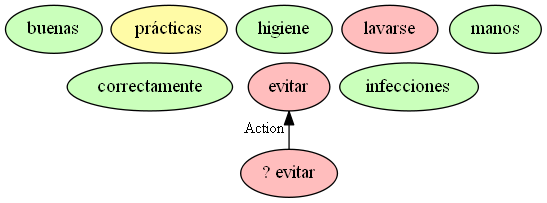
\includegraphics[width=4.2in]{graphics/knowledge_graph_example2_2.png}
		\caption[Ejemplo 2: grafo de conocimiento luego de realizado el punto 2]{Ejemplo 2: grafo de conocimiento luego de realizado el punto 2.}
		\label{fig:knowledge_graph2.2}
	\end{center}
\end{figure}

Una vez completado el punto $3$, este es el resultado:
\begin{figure}[H]
	\begin{center}
		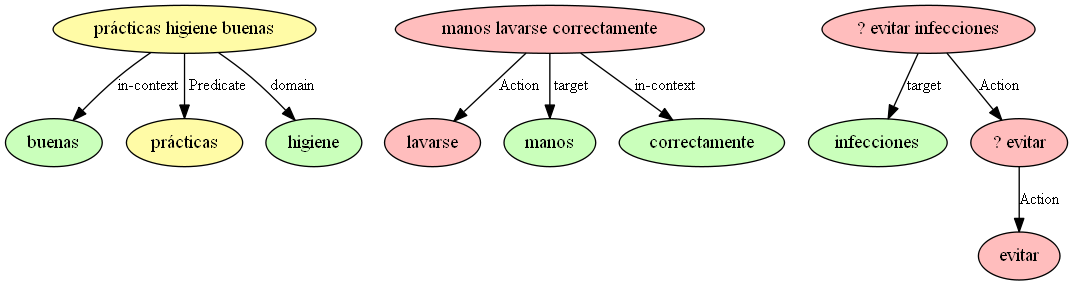
\includegraphics[width=\textwidth]{graphics/knowledge_graph_example2_3.png}
		\caption[Ejemplo 2: grafo de conocimiento luego de realizado el punto 3]{Ejemplo 2: grafo de conocimiento luego de realizado el punto 3.}
		\label{fig:knowledge_graph2.3}
	\end{center}
\end{figure}

Finalmente, al llevar a cabo el punto $4$, este sería el resultado:
\begin{figure}[H]
	\begin{center}
		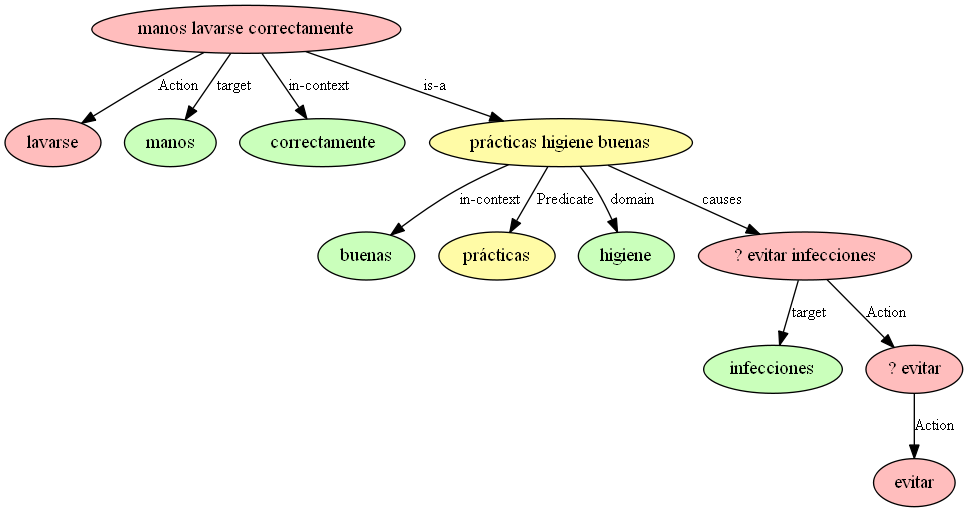
\includegraphics[width=\textwidth]{graphics/knowledge_graph_example2_4.png}
		\caption[Ejemplo 2: grafo de conocimiento luego de realizado el punto 4]{Ejemplo 2: grafo de conocimiento luego de realizado el punto 4.}
		\label{fig:knowledge_graph2.4}
	\end{center}
\end{figure}

Como pudo apreciarse en el ejemplo anterior, se optó por mostrar los atributos en el grafo a través de caracteres en vez de la palabra en sí. Son usados los siguientes caracteres:
\begin{itemize}
	\item[$\lnot$] negación
	\item[?] incertidumbre
	\item[$\downarrow$] disminución
	\item[$\uparrow$] énfasis
\end{itemize}

% {
	% \small
	% $\begin{array}{rrcl}
	% 	1. & \nonterminal{DOCUMENT} & \rightarrow & \varepsilon\\
	% 	\vspace{0.1in}
	% 	&& \vert & \nonterminal{LINE}\nonterminal{NEW\_LINES}\\
	% 	2. & \nonterminal{NEW\_LINES} & \rightarrow & \varepsilon\\
	% 	\vspace{0.1in}
	% 	&& \vert & \nonterminal{NEW\_LINE}\nonterminal{NEW\_LINE\_OR\_DOCUMENT}\\
	% 	3. & \nonterminal{NEW\_LINE\_OR\_DOCUMENT} & \rightarrow & \nonterminal{NEW\_LINES}\\
	% 	\vspace{0.1in}
	% 	&& \vert & \nonterminal{DOCUMENT}\\
	% 	4. & \nonterminal{LINE} & \rightarrow & \nonterminal{ATTRIBUTE}\\
	% 	&& \vert & \nonterminal{COMMENT}\\
	% 	&& \vert & \nonterminal{RELATION}\\
	% 	\vspace{0.1in}
	% 	&& \vert & \nonterminal{TEXT}\\
	% 	5. & \nonterminal{ATTRIBUTE} & \rightarrow & \nonterminal{ATTRIBUTE\_ID}\nonterminal{TAB}\\
	% 	\vspace{0.1in}
	% 	&&& \nonterminal{ATTRIBUTE\_TYPE}\nonterminal{SPACE}\nonterminal{TEXT\_ID}\\
	% 	\vspace{0.1in}
	% 	6. & \nonterminal{COMMENT} & \rightarrow & \nonterminal{COMMENT\_ID}\nonterminal{SPACE}\nonterminal{COMMENT\_TEXT}\\
	% 	7. & \nonterminal{RELATION} & \rightarrow & \nonterminal{RELATION\_ID}\nonterminal{TAB}\\
	% 	&&& \nonterminal{RELATION\_TYPE}\nonterminal{SPACE}\\
	% 	\vspace{0.1in}
	% 	&&& \nonterminal{ARGUMENT1}\nonterminal{SPACE}\nonterminal{ARGUMENT2}\\
	% 	8. & \nonterminal{TEXT} & \rightarrow & \nonterminal{TEXT\_ID}\nonterminal{TAB}\nonterminal{TEXT\_TYPE}\nonterminal{SPACE}\\
	% 	\vspace{0.1in}
	% 	&&& \nonterminal{TEXT\_SPAN}\nonterminal{TAB}\nonterminal{TEXT\_ANNOTATED}\\
	% 	\vspace{0.1in}
	% 	9. & \nonterminal{NEW\_LINE} & \rightarrow & \verb|`\n'|\\
	% 	\vspace{0.1in}
	% 	10. & \nonterminal{TAB} & \rightarrow & \verb|`\t'|\\
	% 	\vspace{0.1in}
	% 	12. & \nonterminal{SPACE} & \rightarrow & \verb|` '|\\
	% 	\vspace{0.1in}
	% 	13. & \nonterminal{ATTRIBUTE\_ID} & \rightarrow & \nonterminal{A}\nonterminal{NUMBER}\\
	% 	14. & \nonterminal{ATTRIBUTE\_TYPE} & \rightarrow & \nonterminal{N}\nonterminal{E}\nonterminal{G}\nonterminal{A}\nonterminal{T}\nonterminal{E}\nonterminal{D}\\
	% 	&& \vert & \nonterminal{U}\nonterminal{N}\nonterminal{C}\nonterminal{E}\nonterminal{R}\nonterminal{T}\nonterminal{A}\nonterminal{I}\nonterminal{N}\\
	% 	&& \vert & \nonterminal{D}\nonterminal{I}\nonterminal{M}\nonterminal{I}\nonterminal{N}\nonterminal{I}\nonterminal{S}\nonterminal{H}\nonterminal{E}\nonterminal{D}\\
	% 	\vspace{0.1in}
	% 	&& \vert & \nonterminal{E}\nonterminal{M}\nonterminal{P}\nonterminal{H}\nonterminal{A}\nonterminal{S}\nonterminal{I}\nonterminal{Z}\nonterminal{E}\nonterminal{D}\\
	% 	15. & \nonterminal{COMMENT\_ID} & \rightarrow & \#\\
	% 	\vspace{0.1in}
	% 	&& \vert & \#\nonterminal{NUMBER}\\
	% 	16. & \nonterminal{COMMENT\_TEXT} & \rightarrow & \varepsilon\\
	% 	\vspace{0.1in}
	% 	&& \vert & \nonterminal{ALPHABET}\nonterminal{COMMENT\_TEXT}\\
	% 	17. & \nonterminal{RELATION\_ID} & \rightarrow & \nonterminal{R}\nonterminal{NUMBER}\\
	% \end{array}$

	% $\begin{array}{rrcl}
	% 	17. & \nonterminal{RELATION\_TYPE} & \rightarrow & \nonterminal{S}\nonterminal{U}\nonterminal{B}\nonterminal{J}\nonterminal{E}\nonterminal{C}\nonterminal{T}\\
	% 	&& \vert & \nonterminal{T}\nonterminal{A}\nonterminal{R}\nonterminal{G}\nonterminal{E}\nonterminal{T}\\
	% 	&& \vert & \nonterminal{D}\nonterminal{O}\nonterminal{M}\nonterminal{A}\nonterminal{I}\nonterminal{N}\\
	% 	&& \vert & \nonterminal{A}\nonterminal{R}\nonterminal{G}\nonterminal{U}\nonterminal{M}\nonterminal{E}\nonterminal{N}\nonterminal{T}\\
	% 	&& \vert & \nonterminal{I}\nonterminal{S}\texttt{-}\nonterminal{A}\\
	% 	&& \vert & \nonterminal{P}\nonterminal{A}\nonterminal{R}\nonterminal{T}\texttt{-}\nonterminal{O}\nonterminal{F}\\
	% 	&& \vert & \nonterminal{S}\nonterminal{A}\nonterminal{M}\nonterminal{E}\texttt{-}\nonterminal{A}\nonterminal{S}\\
	% 	&& \vert & \nonterminal{H}\nonterminal{A}\nonterminal{S}\texttt{-}\nonterminal{P}\nonterminal{R}\nonterminal{O}\nonterminal{P}\nonterminal{E}\nonterminal{R}\nonterminal{T}\nonterminal{Y}\\
	% 	&& \vert & \nonterminal{C}\nonterminal{A}\nonterminal{U}\nonterminal{S}\nonterminal{E}\nonterminal{S}\\
	% 	&& \vert & \nonterminal{E}\nonterminal{N}\nonterminal{T}\nonterminal{A}\nonterminal{I}\nonterminal{L}\nonterminal{S}\\
	% 	&& \vert & \nonterminal{I}\nonterminal{N}\texttt{-}\nonterminal{T}\nonterminal{I}\nonterminal{M}\nonterminal{E}\\
	% 	&& \vert & \nonterminal{I}\nonterminal{N}\texttt{-}\nonterminal{P}\nonterminal{L}\nonterminal{A}\nonterminal{C}\nonterminal{E}\\
	% 	\vspace{0.1in}
	% 	&& \vert & \nonterminal{I}\nonterminal{N}\texttt{-}\nonterminal{C}\nonterminal{O}\nonterminal{N}\nonterminal{T}\nonterminal{E}\nonterminal{X}\nonterminal{T}\\
	% 	\vspace{0.1in}
	% 	17. & \nonterminal{ARGUMENT1} & \rightarrow & \texttt{Arg1:}\nonterminal{TEXT\_ID}\\
	% 	\vspace{0.1in}
	% 	17. & \nonterminal{ARGUMENT2} & \rightarrow & \texttt{Arg2:}\nonterminal{TEXT\_ID}\\
	% 	\vspace{0.1in}
	% 	17. & \nonterminal{TEXT\_ID} & \rightarrow & \nonterminal{T}\nonterminal{NUMBER}\\
	% 	17. & \nonterminal{TEXT\_TYPE} & \rightarrow & \nonterminal{C}\nonterminal{O}\nonterminal{N}\nonterminal{C}\nonterminal{E}\nonterminal{P}\nonterminal{T}\\
	% 	&& \vert & \nonterminal{A}\nonterminal{C}\nonterminal{T}\nonterminal{I}\nonterminal{O}\nonterminal{N}\\
	% 	&& \vert & \nonterminal{R}\nonterminal{E}\nonterminal{F}\nonterminal{E}\nonterminal{R}\nonterminal{E}\nonterminal{N}\nonterminal{C}\nonterminal{E}\\
	% 	\vspace{0.1in}
	% 	&& \vert & \nonterminal{P}\nonterminal{R}\nonterminal{E}\nonterminal{D}\nonterminal{I}\nonterminal{C}\nonterminal{A}\nonterminal{T}\nonterminal{E}\\
	% 	17. & \nonterminal{TEXT\_SPAN} & \rightarrow & \nonterminal{NUMBER}\nonterminal{SPACE}\nonterminal{NUMBER}\\
	% 	\vspace{0.1in}
	% 	&& \vert & \nonterminal{NUMBER}\nonterminal{SPACE}\nonterminal{NUMBER}\texttt{;}\nonterminal{TEXT\_SPAN}\\
	% 	17. & \nonterminal{TEXT\_ANNOTATED} & \rightarrow & \nonterminal{CHAR}\\
	% 	&& \vert & \nonterminal{CHAR}\nonterminal{TEXT\_ANNOTATED}\\
	% 	\vspace{0.1in}
	% 	&& \vert & \nonterminal{CHAR}\nonterminal{SPACE}\nonterminal{CHAR}\nonterminal{TEXT\_ANNOTATED}\\
	% 	17. & \nonterminal{NUMBER} & \rightarrow & \nonterminal{DIGIT}\\
	% 	\vspace{0.1in}
	% 	&& \vert & \nonterminal{DIGIT}\nonterminal{NUMBER}\\
	% 	\vspace{0.1in}
	% 	17. & \nonterminal{DIGIT} & \rightarrow & \texttt{0}~\vert~\texttt{1}~\vert~\texttt{2}~\vert~\texttt{3}~\vert~\texttt{4}~\vert~\texttt{5}~\vert~\texttt{6}~\vert~\texttt{7}~\vert~\texttt{8}~\vert~\texttt{9}\\
	% 	% \vspace{0.1in}
	% 	% 17. & \nonterminal{A} & \rightarrow & \texttt{A}~\vert~\texttt{a}\\
	% 	% \vspace{0.1in}
	% 	% 17. & \nonterminal{B} & \rightarrow & \texttt{B}~\vert~\texttt{b}\\
	% 	% \vspace{0.1in}
	% 	% 17. & \nonterminal{C} & \rightarrow & \texttt{C}~\vert~\texttt{c}\\
	% 	% \vspace{0.1in}
	% 	% 17. & \nonterminal{D} & \rightarrow & \texttt{D}~\vert~\texttt{d}\\
	% 	% 17. & \nonterminal{E} & \rightarrow & \texttt{E}~\vert~\texttt{e}\\
	% % \end{array}$

	% % $\begin{array}{rrcl}
	% 	% \vspace{0.1in}
	% 	% 17. & \nonterminal{F} & \rightarrow & \texttt{F}~\vert~\texttt{f}\\
	% 	% \vspace{0.1in}
	% 	% 17. & \nonterminal{G} & \rightarrow & \texttt{G}~\vert~\texttt{g}\\
	% 	% \vspace{0.1in}
	% 	% 17. & \nonterminal{H} & \rightarrow & \texttt{H}~\vert~\texttt{h}\\
	% 	% \vspace{0.1in}
	% 	% 17. & \nonterminal{I} & \rightarrow & \texttt{I}~\vert~\texttt{i}\\
	% 	% \vspace{0.1in}
	% 	% 17. & \nonterminal{J} & \rightarrow & \texttt{J}~\vert~\texttt{j}\\
	% 	% \vspace{0.1in}
	% 	% 17. & \nonterminal{L} & \rightarrow & \texttt{L}~\vert~\texttt{l}\\
	% 	% \vspace{0.1in}
	% 	% 17. & \nonterminal{M} & \rightarrow & \texttt{M}~\vert~\texttt{m}\\
	% 	% \vspace{0.1in}
	% 	% 17. & \nonterminal{N} & \rightarrow & \texttt{N}~\vert~\texttt{n}\\
	% 	% \vspace{0.1in}
	% 	% 17. & \nonterminal{O} & \rightarrow & \texttt{O}~\vert~\texttt{o}\\
	% 	% \vspace{0.1in}
	% 	% 17. & \nonterminal{P} & \rightarrow & \texttt{P}~\vert~\texttt{p}\\
	% 	% \vspace{0.1in}
	% 	% 17. & \nonterminal{R} & \rightarrow & \texttt{R}~\vert~\texttt{r}\\
	% 	% \vspace{0.1in}
	% 	% 17. & \nonterminal{S} & \rightarrow & \texttt{S}~\vert~\texttt{s}\\
	% 	% \vspace{0.1in}
	% 	% 17. & \nonterminal{T} & \rightarrow & \texttt{T}~\vert~\texttt{t}\\
	% 	% \vspace{0.1in}
	% 	% 17. & \nonterminal{U} & \rightarrow & \texttt{U}~\vert~\texttt{u}\\
	% 	% \vspace{0.1in}
	% 	% 17. & \nonterminal{X} & \rightarrow & \texttt{X}~\vert~\texttt{x}\\
	% 	% \vspace{0.1in}
	% 	% 17. & \nonterminal{Y} & \rightarrow & \texttt{Y}~\vert~\texttt{y}\\
	% 	% \vspace{0.1in}
	% 	% 17. & \nonterminal{Z} & \rightarrow & \texttt{Z}~\vert~\texttt{z}\\
	% 	17. & \nonterminal{ALPHABET} & \rightarrow & \nonterminal{CHAR}\\
	% 	&& \vert & \nonterminal{SPACE}\\
	% 	&& \vert & \nonterminal{TAB}
	% \end{array}$
% \section{Construcción del grafo}